\documentclass[12pt]{article}


\usepackage[utf8]{inputenc}
\usepackage[T1]{fontenc}
\usepackage[polish]{babel}
\usepackage{graphicx}

\usepackage{float}

\title{Sprawozdanie z ćwiczenia A3}
\author{ 
Dawid Legutki \and Piotr Merynda \and Damian Paciuch \and Maciej Podsiadło \and Łukasz Radzio}
\date{Data ćwiczenia: 16.03.2015}

\newtheorem{Def}{Definicja}

\newcommand{\LT}[1]{\mathcal{L}\{#1\}}
\newcommand{\iLT}[1]{\mathcal{L}^{-1}\{#1\}}
\newcommand{\ZMa}{17}
\begin{document}
\maketitle
\section{Wstęp}
\subsection{Schemat stanowiska}

\begin{figure}[H]
\centering
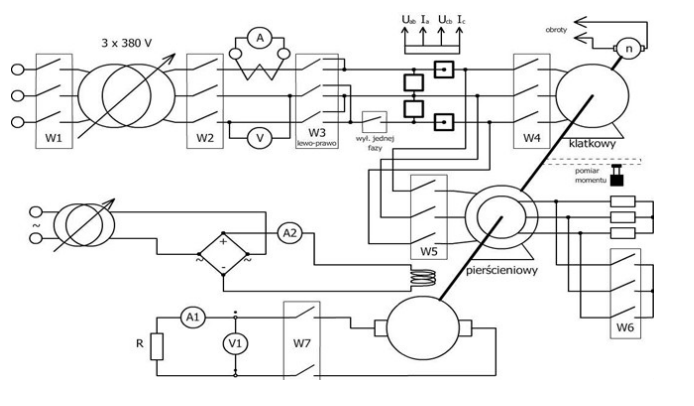
\includegraphics[width=10cm]{schemat_stanowiska}
\end{figure}
\nopagebreak
\subsection{Dane znamionowe silników}
\begin{center}

\begin{tabular}{|c|c|c|}
\hline
	 & \multicolumn{1}{ |c| }{Silnik Klatkowy} 
	 & \multicolumn{1} { |c| }{Silnik Pierścieniowy} \\ 
\hline
	$P_n$ & $3.0kW$ & $4.0kW$ \\
	$U_n$ & $380V$ & $380V$ \\
	$I_n$ & $6.6A$ & $8.5A$ \\
	$n_n$ & $1420$ obr/min & $1435$ obr/min \\
	$\cos\phi$ & $0.81$ & $0.84$ \\
	$R_s$ & $1.2 \Omega$ & $1.26 \Omega$ \\
\hline
\end{tabular}
\end{center}
%\flushleft
\section{Pomiar charakterystyk silnika klatkowego}
\subsection{Charakterystyka mechaniczna}
Z pomiarów otrzymaliśmy napięcie międzyfazowe, prąd przewodowy, prędkość obrotową. Przy stanowisku podana była także wartość momentu bezwładności układu. Moment obrotowy otrzymaliśmy z wzorów:
\begin{equation}
	T_e = J\frac{d\omega}{dt}
\end{equation}
\begin{equation}
	\omega=\frac{2\pi n}{60}
\end{equation}
\begin{equation}
	\frac{d\omega}{dt}\approx\frac{\omega(i+1)-\omega(i)}{t(i+1)-t(i)}
\end{equation}
Pomiary dokonane były przy zaniżonym napięciu zasilającym (w stosunku do znamionowego). Z tego powodu musieliśmy przeskalować wyniki.
\begin{equation}
	T=T_e\left(\frac{U_n}{U}\right)^2
\end{equation}
\subsection{Charakterystyka prądowa}
Zmierzoną wartość prądu przeskalowaliśmy zgodnie z wzorem:
\begin{equation}
	I=I_a\frac{U_n}{U}
\end{equation}
\subsection{Wyniki}
	\begin{figure}[H]
	\centering
	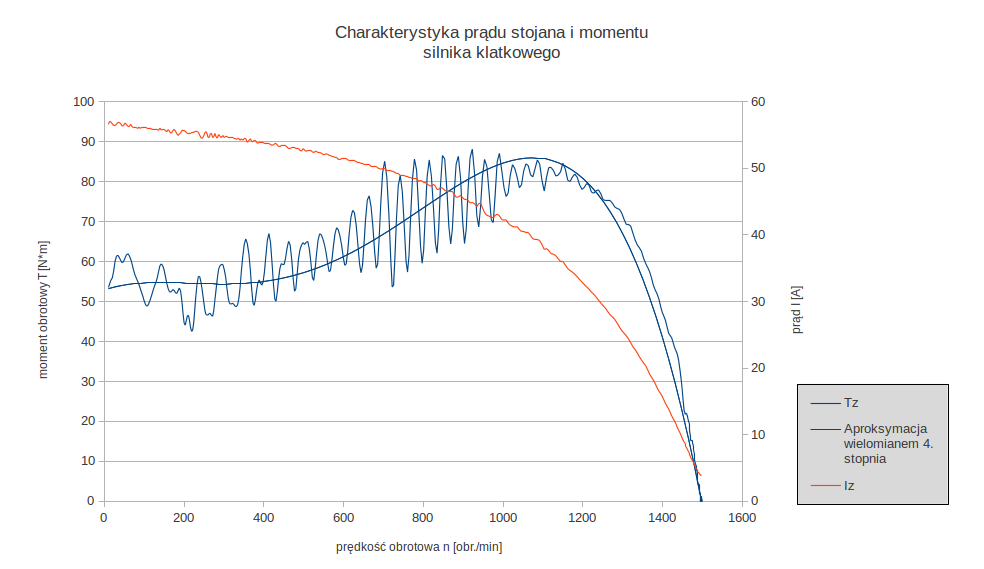
\includegraphics[width=13 cm]{ch_klatkowy}
	\end{figure}
\subsection{Wnioski}
\begin{itemize}
\item Duży prąd rozruchowy
\item Moment rozruchowy większy od zera – zdolność samorozruchu
\item Poślizg krytyczny wynosi około 0,2
\item Prąd rozruchowy dużo większy od znamionowego
\end{itemize}


% \\\\\\\\\\\\\\\\\\\\\\\\\\\\\\\\\\\\\\\\\\\\\\\\\\\\\\\\\\\\\\\\\\\\\\\\\
\section{Pomiar charakterystyk silnika pierścieniowego}
Dokonaliśmy dwóch pomiarów z dodatkową rezystancją podłączoną do wirnika i bez. Wyniki opracowaliśmy w identyczny sposób jak dla silnika klatkowego.
\subsection{Wyniki}
	\begin{figure}[H]
	\centering
	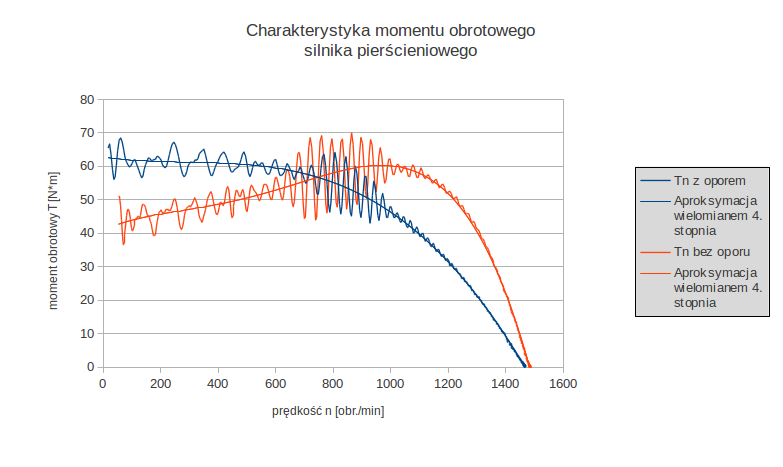
\includegraphics[width=\ZMa cm]{ch_mechaniczna_pierscieniowy}
	\end{figure}
\paragraph{Wpływ podłączenia dodatkowego oporu na ch. mechaniczną:}
\begin{itemize}
	\item Zwiększenie momentu rozruchowego
	\item Zwiększenie poślizgu krytycznego
	\item Przesunięcie charakterystyki w lewo przy zachowaniu prędkości synchronicznej
\end{itemize}
	\begin{figure}[H]
	\centering
	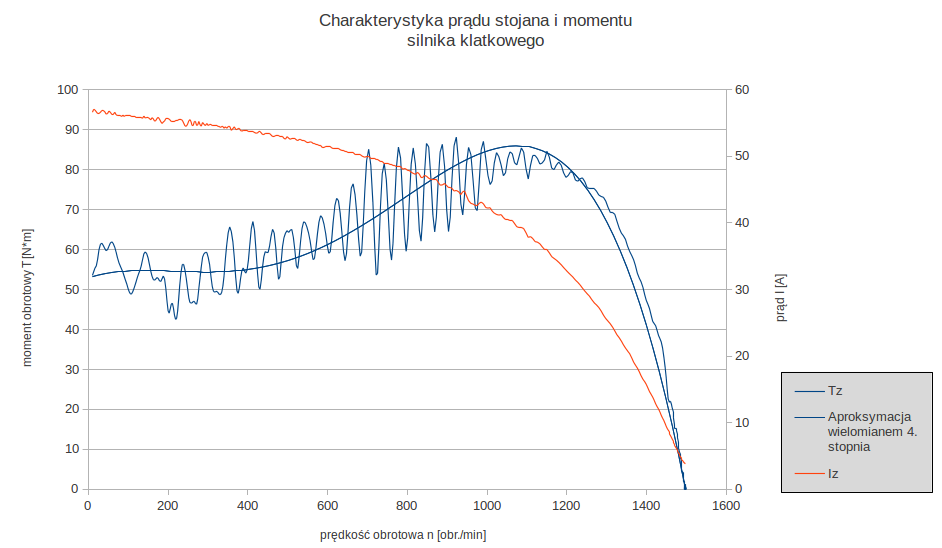
\includegraphics[width=\ZMa cm]{ch_pradowa_pierscieniowy}
	\end{figure}
\paragraph{Wpływ podłączenia dodatkowego oporu na ch. prądową:}
	\begin{itemize}
	\item Zmniejszenie prądu rozruchowego
	\item Przesunięcie charakterystyki w dół
\end{itemize}

\section{Próba biegu jałowego}
	\subsection{Tabela z pomiarami}
		\begin{figure}[H]
			\centering
			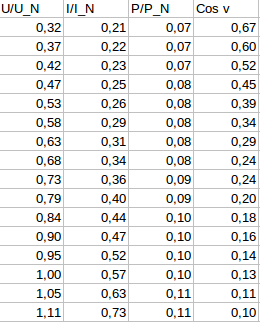
\includegraphics[width=7cm]{jalowy_tab}
		\end{figure}
Po wykonaniu pomiarów zweryfikowaliśmy poprawność wyników:
\begin{equation}
	P=\sqrt{3}IU\cos{\phi}
\end{equation}
Powyższe równanie jest spełnione przez dane pomiarowe.\newline
Następnie dokonaliśmy bilansu mocy:
\begin{equation}
	P=P_{Cu}+P_{Fe}+P_{m}+P_{wir} + P_2 \approx P_{Cu} + P_{m} + P_{Fe}
\end{equation}
Gdzie poszczególne moce oznaczają kolejno straty w miedzi(obwodzie stojana), żelazie(obwodzie magnetycznym), mechaniczne(na łożyskach), straty w obwodzie wirnika i moc użyteczną. Dla próby biegu jałowego moc użyteczna wynosi zero, ponieważ nie obciążamy silnika żadnym dodatkowym momentem(cała moc idzie na utrzymanie ruchu, straty). Ze względu na to że silnik porusza się z prędkością zbliżoną do synchronicznej w obwodzie wirnika płynie pomijalny prąd.
\begin{equation}
	P_{Cu}=3R_sI^2
\end{equation}
\subsection{Charakterystyka mocy}
	\begin{figure}[H]
			\centering
			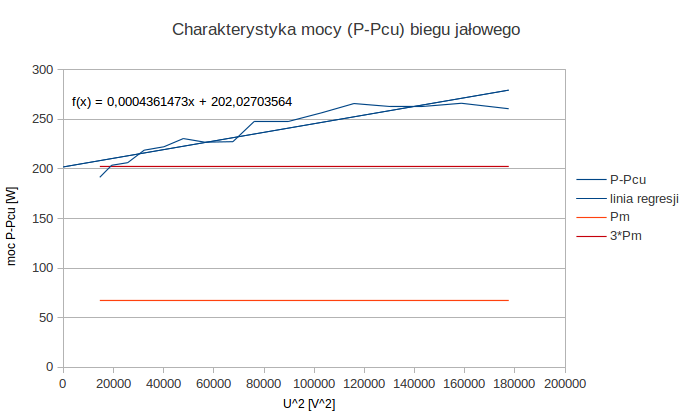
\includegraphics[width=\ZMa cm]{jalowy_moc}
	\end{figure}
Z wykresu otrzymaliśmy wartość strat mechanicznych oraz zależność strat w żelazie od kwadratu napięcia.
\begin{equation}
	P_m=202W
\end{equation}
\begin{equation}
	P_{Fe}=0.00044U^2
\end{equation}

\section{Wyznaczenie charakterystyki obciążeniowej}
\subsection{Tabela z pomiarami}
	\begin{figure}[H]
			\centering
			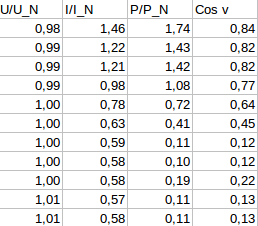
\includegraphics[width=7cm]{obciazenie_tab}
	\end{figure}
	
Bilans mocy dany jest równaniem 7, ale tym razem $P_2$ nie równa się zero nie można też pominąć $P_{wir}$
\begin{equation}
	P_{wir}=(P-P_{Cu}-P_{Fe})s_n
\end{equation}
\begin{equation}
	P_2=P-P_{Cu}-P_{Fe}-P_{m}-P_{wir}-\Delta P_{dodatkowe}
\end{equation}	
$\Delta P_{dodatkowe}$ wynosi $0.5\%$ $P$
%\subsection{Wyniki}
%	\begin{figure}[H]
%			\centering
%			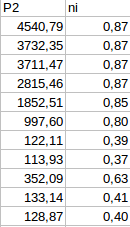
\includegraphics[width=3cm]{wyniki_tab}
%	\end{figure}
\nopagebreak
	\begin{figure}[H]
			\centering
			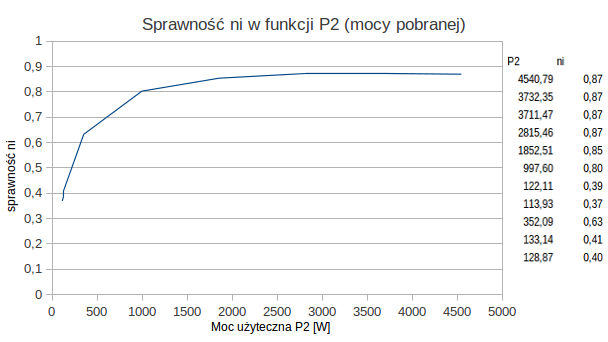
\includegraphics[width=12 cm]{ch_obciazeniowa2}
	\end{figure}
\end{document}



